\documentclass[10pt,dvipdfmx]{beamer}
\usepackage{pgfpages}
\usepackage{graphicx}
\usepackage{listings,jlisting}
\usepackage{fancybox}
\usepackage{hyperref}
\usepackage{multimedia}

%%%%%%%%%%%%%%%%%%%%%%%%%%%
%%% themes
%%%%%%%%%%%%%%%%%%%%%%%%%%%
\usetheme{Rochester}
%% no navigation bar
% default boxes Bergen Boadilla Madrid Pittsburgh Rochester
%% tree-like navigation bar
% Antibes JuanLesPins Montpellier
%% toc sidebar
% Berkeley PaloAlto Goettingen Marburg Hannover Berlin Ilmenau Dresden Darmstadt Frankfurt Singapore Szeged
%% Section and Subsection Tables
% Copenhagen Luebeck Malmoe Warsaw

%%%%%%%%%%%%%%%%%%%%%%%%%%%
%%% innerthemes
%%%%%%%%%%%%%%%%%%%%%%%%%%%
% \useinnertheme{circles}	% default circles rectangles rounded inmargin

%%%%%%%%%%%%%%%%%%%%%%%%%%%
%%% outerthemes
%%%%%%%%%%%%%%%%%%%%%%%%%%%
% outertheme
% \useoutertheme{default}	% default infolines miniframes smoothbars sidebar sprit shadow tree smoothtree


%%%%%%%%%%%%%%%%%%%%%%%%%%%
%%% colorthemes
%%%%%%%%%%%%%%%%%%%%%%%%%%%
\usecolortheme{seahorse}
%% special purpose
% default structure sidebartab 
%% complete 
% albatross beetle crane dove fly seagull 
%% inner
% lily orchid rose
%% outer
% whale seahorse dolphin

%%%%%%%%%%%%%%%%%%%%%%%%%%%
%%% fontthemes
%%%%%%%%%%%%%%%%%%%%%%%%%%%
\usefonttheme{serif}  
% default professionalfonts serif structurebold structureitalicserif structuresmallcapsserif

%%%%%%%%%%%%%%%%%%%%%%%%%%%
%%% generally useful beamer settings
%%%%%%%%%%%%%%%%%%%%%%%%%%%
% 
\AtBeginDvi{\special{pdf:tounicode EUC-UCS2}}
% do not show navigation
\setbeamertemplate{navigation symbols}{}
% show page numbers
\setbeamertemplate{footline}[frame number]


%%%%%%%%%%%%%%%%%%%%%%%%%%%
%%% define some colors for convenience
%%%%%%%%%%%%%%%%%%%%%%%%%%%

\newcommand{\mido}[1]{{\color{green}#1}}
\newcommand{\mura}[1]{{\color{purple}#1}}
\newcommand{\ore}[1]{{\color{orange}#1}}
\newcommand{\ao}[1]{{\color{blue}#1}}
\newcommand{\aka}[1]{{\color{red}#1}}

\setbeamercolor{syntax}{bg=cyan!20!white}
\setbeamercolor{example}{bg=yellow!20!white}
\setbeamercolor{output}{bg=white}

%%%%%%%%%%%%%%%%%%%%%%%%%%%
%%% how to typset code
%%%%%%%%%%%%%%%%%%%%%%%%%%%

\lstset{language = python,
numbers = left,
numberstyle = {\tiny \emph},
numbersep = 10pt,
breaklines = true,
breakindent = 40pt,
frame = tlRB,
frameround = ffft,
framesep = 3pt,
rulesep = 1pt,
rulecolor = {\color{blue}},
rulesepcolor = {\color{blue}},
flexiblecolumns = true,
keepspaces = true,
basicstyle = \ttfamily\small,
identifierstyle = ,
commentstyle = ,
stringstyle = ,
showstringspaces = false,
tabsize = 4,
escapechar=\@,
xrightmargin=3zw,
}


\title{Visual Python, Numpy, Matplotlib}
\institute{東京大学}
\author{田浦健次朗 \\ 電子情報工学科}
\date{}

\AtBeginSection[] % Do nothing for \section*
{
\begin{frame}
\frametitle{Contents}
\tableofcontents[currentsection,currentsubsection]
\end{frame}
}

\begin{document}
\maketitle

%%%%%%%%%%%%%%%%%%%%%%%%%%%%%%%%%% 
\begin{frame}
\frametitle{Contents}
\tableofcontents
\end{frame}

%%%%%%%%%%%%%%%%% %%%%%%%%%%%%%%%%% 
\section{イントロ}
%%%%%%%%%%%%%%%%% %%%%%%%%%%%%%%%%% 

%%%%%%%%%%%%%%%%% %%%%%%%%%%%%%%%%% 
\begin{frame}
\frametitle{3つの飛び道具}
\begin{itemize}
\item Visual Python: 3Dアニメーションを超お手軽に
\item Numpy, Scipy: 高度な行列・ベクトル計算や数値計算を一言で呼び出し
\item Matplotlib: 関数やデータの可視化(グラフ化)
\end{itemize}
\end{frame}


%%%%%%%%%%%%%%%%% %%%%%%%%%%%%%%%%% 
\section{Visual Python}
%%%%%%%%%%%%%%%%% %%%%%%%%%%%%%%%%% 

%%%%%%%%%%%%%%%%% %%%%%%%%%%%%%%%%% 
\begin{frame}[fragile]
\frametitle{シミュレーションから可視化まで}

\begin{enumerate}
\item シミュレーション(数値計算)をする
\item vectorで3D世界の計算にする
\item Visual Pythonのオブジェを作ればできあがり
\end{enumerate}

\end{frame}


%%%%%%%%%%%%%%%%% %%%%%%%%%%%%%%%%% 
\begin{frame}[fragile]
\frametitle{1つの質点のシミュレーションのテンプレート}
要するにこれだけ

\begin{lstlisting}
n_steps = ステップ数
dt = (@\ao{終了時刻}@ - @\ao{開始時刻}@) / n_steps # 時間の刻み幅
x = @\ao{初期位置}@
v = @\ao{初速}@
t = @\ao{開始時刻}@
for i in range(n_steps):
    alpha = @\aka{力}@ / 質量  # 加速度
    x += v * dt       # 位置 += 速度 * 時間
    v += alpha * dt   # 速度 += 加速度 * 時間
    t += dt
\end{lstlisting}

\begin{itemize}
\item \aka{赤字}が問題によって本質的に変わる部分.
\aka{力}を, t, x, vの式で書ければ実質的な仕事は終了
\item \ao{青字}は問題設定によって決まる
\item ステップ数は, 欲しい精度に応じて決める
\end{itemize}
\end{frame}

%%%%%%%%%%%%%%%%% %%%%%%%%%%%%%%%%% 

\begin{frame}[fragile]
\frametitle{適用例 : 吊るされたバネ}
\begin{itemize}
\item バネが自然長のときの重りの位置を $y = 0$ とする
\item 時刻$t = 0$から$10$までシミュレーションするとする
\item 初期位置 $y = 0$, 初速 $v = 0$ とする
\item \aka{力} : $-ky + mg$  ($g=-0.98$)
\item 注: 以下の例で$t$は力の計算に不要なので,
  計算から削除している
\end{itemize}

\begin{lstlisting}
k = 1.0
g = -9.8
m = 1.0
n_steps = 1000
dt = (10.0 - 0) / n_steps 
y = 0.0
v = 0.0
for i in range(n_steps):
    alpha = -k * y / m + g
    y += v * dt
    v += alpha * dt
\end{lstlisting}

\end{frame}


%%%%%%%%%%%%%%%%% %%%%%%%%%%%%%%%%% 

\begin{frame}[fragile]
\frametitle{3D世界の計算にする}
\begin{itemize}
\item 数値の代わりに\aka{Visual Pythonのvectorを使う} $\rightarrow$
  ほとんど変更なく各値をベクトルにできる
\item 注: もちろんこの例においては運動自身は一次元内の運動なので,
  本質的な意味はない
\end{itemize}

\begin{lstlisting}
@\mura{\tt from vpython import *}@
k = 1.0
g = @\mura{\tt vector(0.0, -9.8, 0.0)}@
m = 1.0
n_steps = 1000
dt = (10.0 - 0) / n_steps 
y = @\mura{\tt vector(0.0, 0.0, 0.0)}@
v = @\mura{\tt vector(0.0, 0.0, 0.0)}@
for i in range(n_steps):
    alpha = -k * y /m + g
    y += v * dt
    v += alpha * dt
\end{lstlisting}
\end{frame}


%%%%%%%%%%%%%%%%% %%%%%%%%%%%%%%%%% 

\begin{frame}[fragile]
\frametitle{アニメ化}
\begin{itemize}
\item 位置をVisual Pythonのオブジェクトのposにセットするだけ
\item 速度や加速度も適宜オブジェクトの属性にするとわかりやすい
\item 注: 以下ではバネ(helix)は表示していない
\end{itemize}

\begin{lstlisting}
from vpython import *
k = 1.0
g = vector(0.0, -9.8, 0.0)
m = 1.0
n_steps = 1000
dt = (10.0 - 0) / n_steps
cv = canvas()
@\mura{\tt s = sphere(pos=vector(0.0, 0.0, 0.0))}@
@\mura{\tt s.vel}@ = vector(0.0, 0.0, 0.0)
cv.autoscale = 0 # 場合によりけり
cv.autocenter = 0 # 場合によりけり
for i in range(n_steps):
    rate(1.0/dt)
    @\aka{\tt s.alpha}@ = -k * @\aka{\tt s.pos}@ /m + g
    @\aka{\tt s.pos}@ += @\aka{\tt s.vel}@ * dt
    @\aka{\tt s.vel}@ += @\aka{\tt s.alpha}@ * dt
\end{lstlisting}
\end{frame}

%%%%%%%%%%%%%%%%% %%%%%%%%%%%%%%%%% 

\begin{frame}[fragile]
\frametitle{アニメーション化する際のいくつかのトラップ}

\begin{itemize}
\item rate($f$) : これを時々よばないと(posを変更しても)画面は更新されない
  \begin{itemize}
  \item $f$ : 更新頻度が1秒$f$程度になるよう時間調整
  \end{itemize}

\item カメラの自動追随機能により,動いているオブジェクトが動いているように見えないことがある(例えば1個しかオブジェクトがない場合に顕著)
  \begin{itemize}
  \item 解1: 動かないオブジェクト(板とか)も何か表示する
  \item 解2: 初期状態を表示し終えたところで,以下のおまじないをとなえる
\begin{lstlisting}
cv = canvas()
   ...
# 初期配置完了したあたりで
cv.autocenter = 0 
cv.autoscale = 0      
\end{lstlisting}
  \end{itemize}
\end{itemize}
\end{frame}

%%%%%%%%%%%%%%%%% %%%%%%%%%%%%%%%%% 

\begin{frame}[fragile]
\frametitle{物体が複数の場合}

\begin{itemize}
\item 基本: 物体一つにつき位置, 速度などの変数を1セット
\item 簡単な場合は, 物体1つ $=$ Visual Pythonのオブジェクト一つ
\item 物体が増えてきたらリストなどを使う
\end{itemize}

\end{frame}


%%%%%%%%%%%%%%%%% %%%%%%%%%%%%%%%%% 
\section{NumpyとScipy}
%%%%%%%%%%%%%%%%% %%%%%%%%%%%%%%%%% 
\begin{frame}
\frametitle{NumpyとScipy}
\begin{itemize}
\item SciPy
\item NumPy (Numerical Python)
\item NumPy $\subset$ SciPy ということのようだ
\item numpyで提供されている機能は{\bf そのまま}, 
  scipyでも提供されている
\item なのでscipyだけで押し通しても良さそうだが,
  世の中の説明はnumpyが主流なので, それに合わせて,
  基本はnumpy, scipyだけで提供されている機能はscipyを使う
\end{itemize}

\end{frame}

\iffalse
%%%%%%%%%%%%%%%%% %%%%%%%%%%%%%%%%% 
\begin{frame}[fragile]
\frametitle{インストール \& お試し}

\begin{lstlisting}
$ @{\bf sudo apt-get install python-numpy python-scipy}@
$ @{\bf python}@
 ...
>>> @{\bf import numpy}@
>>> @{\bf numpy.array([2,0,1,4])}@
array([2, 0, 1, 4])
\end{lstlisting} % 
\end{frame}

%%%%%%%%%%%%%%%%% %%%%%%%%%%%%%%%%% 
\begin{frame}[fragile]
\frametitle{もっとあるimportの仕方}
\begin{itemize}
\item 方法1: 
\begin{lstlisting}
>>> @{\bf import numpy}@
>>> @{\bf\aka{numpy.}array([2,0,1,4])}@ # 毎回 numpy. をつける
\end{lstlisting}
\begin{itemize}
\item 安全かつわかりやすい
\item タイプの手間が大きい
\end{itemize}

\item 方法2:
\begin{lstlisting}
>>> from numpy import *
>>> array([2,0,1,4])
\end{lstlisting}
\begin{itemize}
\item タイプの手間が少ない
\item たくさんのimportをすると名前の衝突の可能性があり, 混乱の元
  (vpython.rate と numpy.rate)
\end{itemize}
\end{itemize}
\end{frame}

%%%%%%%%%%%%%%%%% %%%%%%%%%%%%%%%%% 
\begin{frame}[fragile]
\frametitle{もっとあるimportの仕方}
\begin{itemize}
\item 方法3:
\begin{lstlisting}
>>> @\aka{import numpy as np}@
>>> @\aka{np.}@array([2,0,1,4])
\end{lstlisting}
\begin{itemize}
\item タイプの手間も少なく, 名前の衝突の心配もない. 
  世の中のnumpyの例題でも多用されている
\end{itemize}

\item 方法4 (選択的にimport):
\begin{lstlisting}
>>> @\aka{from numpy import array}@
>>> array([2,0,1,4])
\end{lstlisting}
\end{itemize}

以下の説明では方法3を用いる.

\end{frame}
\fi

%%%%%%%%%%%%%%%%% %%%%%%%%%%%%%%%%% 
\begin{frame}[fragile]
\frametitle{有用なチュートリアル}
\begin{itemize}
\item 以下ではspeed learningのために基本を駆け足で説明する
\item 適宜, 以下のページなどを参照すると良い
\url{http://wiki.scipy.org/Tentative_NumPy_Tutorial}
\end{itemize}

\end{frame}

%%%%%%%%%%%%%%%%% %%%%%%%%%%%%%%%%% 
\begin{frame}[fragile]
\frametitle{array : numpyの基本データ}
\begin{itemize}
\item numpyの中心データは, {\tt array}
\item arrayを作る:
\begin{lstlisting}
import numpy as np
np.array(リスト)
\end{lstlisting}
\item 例:
\begin{lstlisting}
import numpy as np
x = @\aka{np.array([2,0,1,4])}@
print(x)
print(len(x))
print(x[1])
\end{lstlisting}

\item 出力:
\begin{lstlisting}
[2 0 1 4]
4
0
\end{lstlisting}
\end{itemize}
\end{frame}


%%%%%%%%%%%%%%%%% %%%%%%%%%%%%%%%%% 
\begin{frame}[fragile]
\frametitle{多次元のarray}
\begin{itemize}
\item 例:
\begin{lstlisting}
import numpy as np
A = @\aka{np.array([[1,2,3],[4,5,6]])}@
print(A)
print(len(A))
print(A[1][1])
\end{lstlisting}

\item 出力:
\begin{lstlisting}
[[1 2 3]
 [4 5 6]]
2
5
\end{lstlisting}

\item 想像通り, 3次元, 4次元, \ldots のarrayも作れる
\end{itemize}
\end{frame}

%%%%%%%%%%%%%%%%% %%%%%%%%%%%%%%%%% 
\begin{frame}[fragile]
\frametitle{arrayの演算}
\begin{itemize}
\item 
\begin{lstlisting}
import numpy as np
x = np.array([2,0,1,4])
y = np.array([5,6,7,8])
print(@\ao{x + y}@)
print(@\aka{x * y}@) # @\aka{注意}@
print(@\ao{x.dot(y)}@)
\end{lstlisting}
\item 
\begin{lstlisting}
@\ao{[ 7  6  8 12]}@
@\aka{[10  0  7 32]}@  # 要素ごとの *
@\aka{49}@             # 内積
\end{lstlisting}
\end{itemize}
\end{frame}

%%%%%%%%%%%%%%%%% %%%%%%%%%%%%%%%%% 
\begin{frame}[fragile]
\frametitle{arrayの演算 (続)}
\begin{itemize}
\item 行列$\times$ベクトル:
\begin{lstlisting}
import numpy
A = numpy.array([[1,2,3],[4,5,6]])
x = numpy.array([2,4,6])
print(@\aka{A.dot(x)}@)
\end{lstlisting}
\begin{lstlisting}
[28 64]
\end{lstlisting}

\item 行列$\times$行列
\begin{lstlisting}
import numpy
A = numpy.array([[1,2,3],[4,5,6]])
B = numpy.array([[2,3],[4,5],[6,7]])
print(@\aka{A.dot(B)}@)
\end{lstlisting}
\begin{lstlisting}
[[28 34]
 [64 79]]
\end{lstlisting}
\end{itemize}
\end{frame}

%%%%%%%%%%%%%%%%% %%%%%%%%%%%%%%%%% 
\begin{frame}[fragile]
\frametitle{matrix : '*' で行列積がしたければ}
\begin{itemize}
\item arrayは任意の次元のデータの集まりを表す, 汎用的なデータで,
「行列」専用というわけではない(その意味で, {\tt *}の動作は自然)
\item 「行列」を使いたければmatrixを使う
\item 
\begin{lstlisting}
import numpy as np
A = np@\aka{.matrix}@([[1,2,3],[4,5,6]])
B = np@\aka{.matrix}@([[2,3],[4,5],[6,7]])
print(@\aka{A * B}@)
\end{lstlisting}
\begin{lstlisting}
[[28 34]
 [64 79]]
\end{lstlisting}

\item そして, arrayを受け付ける関数の殆どは,
matrixも受け付ける
\end{itemize}
\end{frame}

%%%%%%%%%%%%%%%%% %%%%%%%%%%%%%%%%% 
\begin{frame}[fragile]
\frametitle{arrayの色々な作り方 (1) \\
よく使う基本形}

\begin{itemize}
\item 等差数列 (公差を指定)
\begin{lstlisting}
>>> np.@\aka{arange(2,3,0.2)}@
array([ 2. ,  2.2,  2.4,  2.6,  2.8])
\end{lstlisting}

\item 等差数列 (点数を指定)
\begin{lstlisting}
>>> np.@\aka{linspace(2,3,6)}@
array([ 2. ,  2.2,  2.4,  2.6,  2.8,  3. ])
\end{lstlisting}

\item 0や1を並べる
\begin{lstlisting}
>>> np.@\aka{zeros((3,2))}@
array([[ 0.,  0.],
       [ 0.,  0.],
       [ 0.,  0.]])
\end{lstlisting}
\begin{lstlisting}
np.@\aka{ones((2,3))}@
array([[ 1.,  1.,  1.],
       [ 1.,  1.,  1.]])
\end{lstlisting}
\end{itemize}
\end{frame}

%%%%%%%%%%%%%%%%% %%%%%%%%%%%%%%%%% 
\begin{frame}[fragile]
\frametitle{arrayの色々な作り方 (2) \\
つぶしの効くやり方}
\begin{itemize}
\item ややこしい物を作りたければ,
zerosなどで形だけ作り, 各要素に値を代入すれば良い

\begin{lstlisting}
import numpy as np

def make_diag(n):
    A = np.zeros((n,n))
    for i in range(n):
        @\aka{A[i,i] = i + 1}@
    return A

print(make_diag(4))
\end{lstlisting}

\begin{lstlisting}
[[ 1.  0.  0.  0.]
 [ 0.  2.  0.  0.]
 [ 0.  0.  3.  0.]
 [ 0.  0.  0.  4.]]
\end{lstlisting}
\end{itemize}
\end{frame}

%%%%%%%%%%%%%%%%% %%%%%%%%%%%%%%%%% 
\begin{frame}[fragile]
\frametitle{arrayの色々な作り方 (3) \\
reshape}

\begin{itemize}
\item 要素の並びはそのままにして, 形(次元や縦横の要素数)を変える
  \begin{itemize}
  \item ベクトル(1次元) $\leftrightarrow$ 行列(2次元) など
  \item $3\times 5$行列 $\leftrightarrow$ $5\times 3$行列など
  \end{itemize}
\item 
\begin{lstlisting}
A = np.arange(0, 15, 1)@\aka{.reshape(3, 5)}@
print(A)
B = A@\aka{.reshape(5, 3)}@
print(B)
\end{lstlisting}

\begin{lstlisting}
[[ 0  1  2  3  4]
 [ 5  6  7  8  9]
 [10 11 12 13 14]]
[[ 0  1  2]
 [ 3  4  5]
 [ 6  7  8]
 [ 9 10 11]
 [12 13 14]]
\end{lstlisting}
\end{itemize}
\end{frame}

%%%%%%%%%%%%%%%%% %%%%%%%%%%%%%%%%% 
\begin{frame}[fragile]
\frametitle{arrayの色々な作り方 (4)}
その他たまに便利なもの

\begin{itemize}
\item 乱数
\begin{lstlisting}
>>> np@\aka{.random.random((3,3))}@
array([[ 0.1065879 ,  0.99028258,  0.05101186],
       [ 0.33271903,  0.42683107,  0.88456947],
       [ 0.52302174,  0.63007686,  0.84804093]])
\end{lstlisting}

\item 関数で作る
\begin{lstlisting}
>>> def f(I,J):
...   return I + J
... 
>>> np@\aka{.fromfunction(f, (3,3))}@
array([[ 0.,  1.,  2.],
       [ 1.,  2.,  3.],
       [ 2.,  3.,  4.]])
\end{lstlisting}
     
\end{itemize}
\end{frame}


%%%%%%%%%%%%%%%%% %%%%%%%%%%%%%%%%% 
\begin{frame}[fragile]
\frametitle{要素, 行, 列の取り出し}
\begin{itemize}
\item 特定の行, 特定の列など, 自由に切り出すことが可能
\end{itemize}

\begin{lstlisting}
import numpy
A = np.arange(0, 15, 1).reshape(3, 5)
>>> A
array([[ 0,  1,  2,  3,  4],
       [ 5,  6,  7,  8,  9],
       [10, 11, 12, 13, 14]])
>>> A[1,2]
7
>>> A[@\aka{1:3,2:4}@]
array([[ 7,  8],
       [12, 13]])
\end{lstlisting}
\end{frame}

%%%%%%%%%%%%%%%%% %%%%%%%%%%%%%%%%% 
\begin{frame}[fragile]
\frametitle{要素, 行, 列の取り出し}
\begin{lstlisting}
>>> A[1:3,@\aka{:}@]   # @$=$@ A[1:3,0:5]
array([[ 5,  6,  7,  8,  9],
       [10, 11, 12, 13, 14]])
>>> A[@\aka{:}@,2:4]   # @$=$@ A[0:3,2:4]
array([[ 2,  3],
       [ 7,  8],
       [12, 13]])
>>> A[:,2]
array([ 2,  7, 12])
>>> A[:,:]
array([[ 0,  1,  2,  3,  4],
       [ 5,  6,  7,  8,  9],
       [10, 11, 12, 13, 14]])
\end{lstlisting}
\end{frame}


%%%%%%%%%%%%%%%%% %%%%%%%%%%%%%%%%% 
\begin{frame}[fragile]
\frametitle{Universal関数 (1)}
\begin{itemize}
\item 数値に対する演算の多くがひとりでに,
  arrayに拡張されている
\item 
{\small
\begin{lstlisting}
>>> import numpy as np
>>> r = np.linspace(0, 0.5 * math.pi, 6)
>>> r
array([ 0., 0.31415927, 0.62831853, 0.9424778, 1.25663706, 1.57079633])
>>> @\ao{\tt r + 2}@
array([ 2., 2.31415927, 2.62831853, 2.9424778, 3.25663706, 3.57079633])
>>> @\ao{\tt r ** 2}@
array([ 0., 0.09869604, 0.39478418, 0.8882644, 1.5791367, 2.4674011 ])
\end{lstlisting}}
\end{itemize}
\end{frame}

%%%%%%%%%%%%%%%%% %%%%%%%%%%%%%%%%% 
\begin{frame}[fragile]
\frametitle{Universal関数 (2)}
\begin{itemize}
\item また,$\sin$, $\cos$など一部の数学関数は,
mathで提供されているものはarrayに適用不可だが,
arrayにも適用可なものがnumpyで同名で提供されている

\item 
{\small
\begin{lstlisting}
>>> import numpy as np
>>> import math
>>> r = np.linspace(0, 0.5 * math.pi, 6)
>>> @\aka{math.sin(r)}@
Traceback (most recent call last):
  File "<stdin>", line 1, in <module>
TypeError: only length-1 arrays can be converted to Python scalars
>>> np.sin(0.5 * math.pi)
1.0
>>> @\aka{np.sin(r)}@
array([ 0., 0.30901699, 0.58778525, 0.80901699, 0.95105652, 1.        ])
\end{lstlisting}}
\end{itemize}
\end{frame}

%%%%%%%%%%%%%%%%% %%%%%%%%%%%%%%%%% 
\begin{frame}[fragile]
\frametitle{Numpyに備わる飛び道具}
\begin{itemize}
\item 連立一次方程式($Ax=b$)を解く
\begin{lstlisting}
x = np.linalg.solve(A, b)
\end{lstlisting}
\item 固有値,固有ベクトル
\begin{lstlisting}
d,p = np.linalg.eig(A)
\end{lstlisting}
\item 行列式
\begin{lstlisting}
rank = np.linalg.det(A)
\end{lstlisting}
\item ランク
\begin{lstlisting}
rank = np.linalg.matrix_rank(A)
\end{lstlisting}
\item その他いっぱい\ldots
\end{itemize}
\end{frame}

%%%%%%%%%%%%%%%%% %%%%%%%%%%%%%%%%% 
\section{Scipy}
%%%%%%%%%%%%%%%%% %%%%%%%%%%%%%%%%% 
\begin{frame}
\frametitle{Scipy}
\begin{itemize}
\item とにかく色々なことが一撃でできるようになっている
\item 積分(scipy.integrate)
\item 常微分方程式(scipy.odeint)
\item 関数の最大最小(scipy.optimize)
\item \ldots
\item 仮に今回使わなくてもscipyという単語を覚えておくだけで,
  将来きっと役に立つ
\item \url{http://docs.scipy.org/doc/scipy/reference/}
\end{itemize}
\end{frame}


%%%%%%%%%%%%%%%%% %%%%%%%%%%%%%%%%% 
\section{Matplotlib}
%%%%%%%%%%%%%%%%% %%%%%%%%%%%%%%%%% 
\begin{frame}
\frametitle{Matplotlib}
\begin{itemize}
\item データの可視化
\item Visualのような物体の可視化, アニメーションではなく,
データの可視化(グラフ表示)を得意とする
\item Matplotlibにデータを渡すのに, 
  numpyのarray形式で渡す
\item 機能が豊富で, 十数枚のスライドで多くをカバーするのは無謀
\item 基本概念 $+$ 最小限の例を説明する
\end{itemize}
\end{frame}

\begin{frame}
\frametitle{Matplotlib}
後は, 以下のページなどを適宜参照. おそらくこのスライドよりもよほど有用.
\begin{itemize}
\item document全体: \url{http://matplotlib.org/contents.html}
\item user's guide: \url{http://matplotlib.org/users/index.html}
  \begin{itemize}
  \item Pyplot tutorial (一変数関数$y=f(x)$の表示)
  \item mplot3d (3Dで表示したい場合のキーワード)
%  \item Image tutorial (二変数関数$z=f(x,y)$を色などで表示)
  \end{itemize}

\item Gallery (こんな絵はどう書くんだろうと思ったらここから探す)
\url{https://matplotlib.org/gallery/}

\item Plotting Command Summary (色々なグラフの書き方の総覧)
\url{https://matplotlib.org/3.2.1/api/pyplot_summary.html}

\end{itemize}

\end{frame}


\iffalse
%%%%%%%%%%%%%%%%% %%%%%%%%%%%%%%%%% 
\begin{frame}[fragile]
\frametitle{インストール \& お試し}

\begin{lstlisting}
$ @{\bf sudo apt-get install python-matplotlib python-matplotlib-data }@
$ @{\bf python}@
 ...
>>> import matplotlib.pyplot
>>> matplotlib.pyplot.plot([1,2,3,4],[1,4,9,16])
[<matplotlib.lines.Line2D object at 0x220d850>]
>>> matplotlib.pyplot.show()
\end{lstlisting}
\end{frame}
\fi

%%%%%%%%%%%%%%%%% %%%%%%%%%%%%%%%%% 
\begin{frame}[fragile]
\frametitle{1変数関数($y = f(x)$)をプロットする}

\begin{itemize}
\item 最低限覚えるべき関数: \ao{matplotlib.pyplot}というモジュールの,
\ao{plot}と\ao{show}
\item 長すぎるので普通は,
\begin{lstlisting}
import matplotlib.pyplot as plt
plt.plot(...)
plt.show(...)
\end{lstlisting}

\item 基本概念: \ao{プロットしたいデータ
の$x$座標, $y$座標をそれぞれリストやarrayとして, 
plot関数に渡し, show関数で画面に表示}
\begin{lstlisting}
import matplotlib.pyplot as plt
import numpy as np
x = np.arange(0, 10, 0.1) # [0 0.1 0.2 0.3 .. ]
y = np.sin(x)  # universal関数
# y = [sin(0) sin(0.1) sin(0.2) ... ] 
plt.plot(x, y)
plt.show()
\end{lstlisting}
\end{itemize}
\end{frame}

%%%%%%%%%%%%%%%%% %%%%%%%%%%%%%%%%% 
\begin{frame}[fragile]
\frametitle{1変数関数($y = f(x)$)のプロット例}
\begin{itemize}
\item []
\begin{lstlisting}[basicstyle=\ttfamily\scriptsize]
import matplotlib.pyplot as plt
import numpy as np
x = np.arange(0, 10, 0.1) # [0 0.1 0.2 0.3 .. ]
y = np.sin(x)  # universal関数
# y = [sin(0) sin(0.1) sin(0.2) ... ] 
plt.plot(x, y)
plt.show()
\end{lstlisting}

\item []
\begin{center}
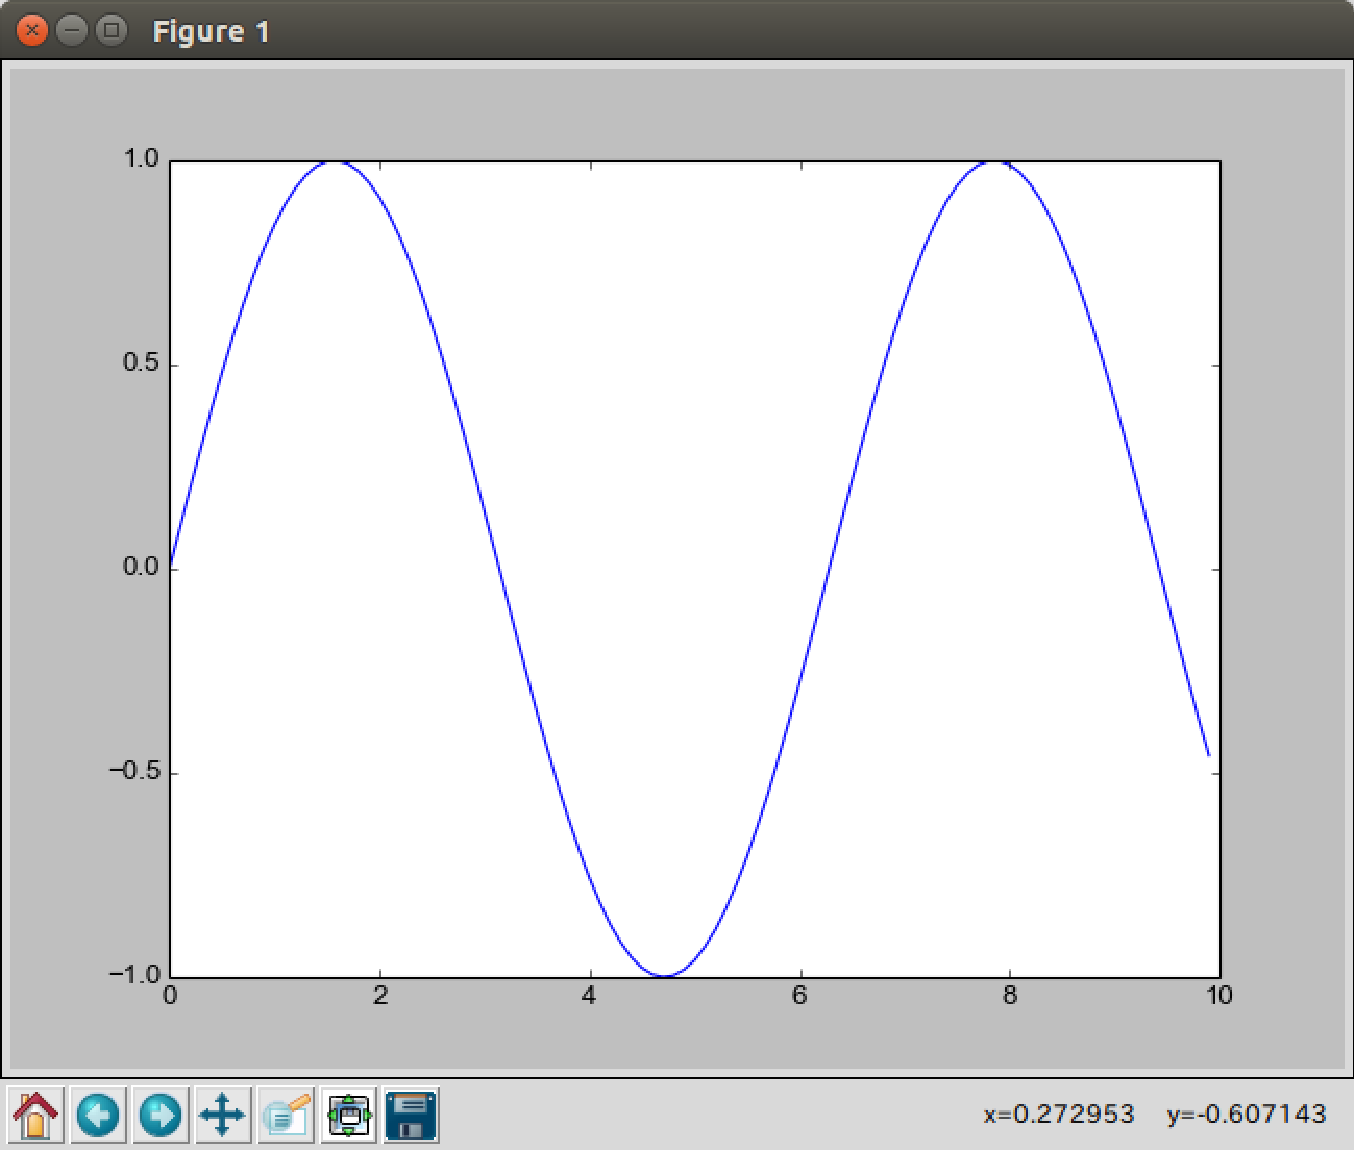
\includegraphics[width=0.5\textwidth]{out/pdf/img/sin.pdf}
\end{center}
\end{itemize}
\end{frame}


\iffalse
%%%%%%%%%%%%%%%%% %%%%%%%%%%%%%%%%% 
\begin{frame}[fragile]
\frametitle{Jupyter環境で表示結果を残す方法}

\begin{columns}
  \begin{column}{0.5\textwidth}
\begin{itemize}
\item 以下のおまじないで,結果がブラウザ内に表示されるようになる
\begin{lstlisting}
%matplotlib inline  
\end{lstlisting}
\begin{itemize}
\item 利点: 結果が残る(記録やプレゼンに便利)
\item 欠点: 拡大・縮小など,操作できない
\end{itemize}

\item 元に戻す
\begin{lstlisting}
%matplotlib
\end{lstlisting}
\end{itemize}
  \end{column}
  \begin{column}{0.5\textwidth}
\begin{center}
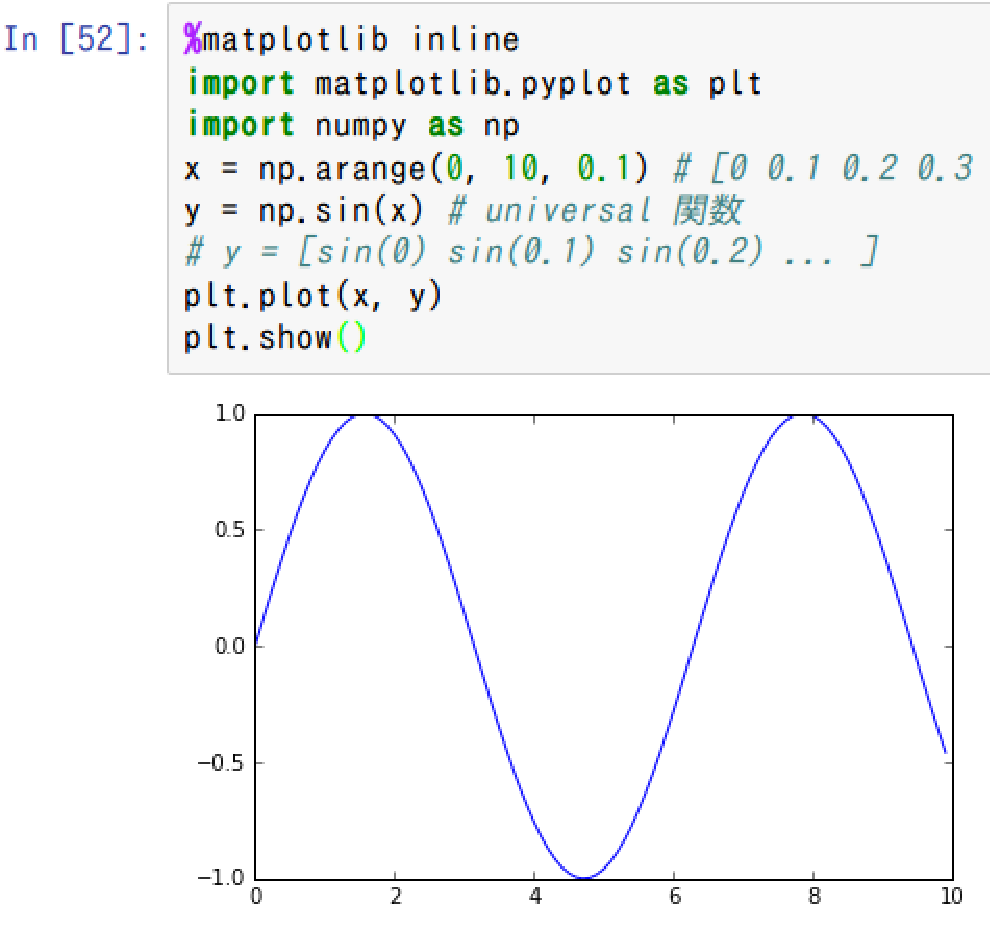
\includegraphics[width=\textwidth]{out/pdf/img/sin_inline.pdf}
\end{center}
  \end{column}
\end{columns}
\end{frame}
\fi

%%%%%%%%%%%%%%%%% %%%%%%%%%%%%%%%%% 
\begin{frame}[fragile]
\frametitle{色々な表示の仕方}
\begin{itemize}
\item とにかく色々な表示の種類(棒グラフ, 散布図, \ldots etc.)
があります
\item {\tt plot}関数の代わりに別の関数を使えば良い
  \begin{itemize}
  \item 棒グラフ$\rightarrow$\ao{\texttt{bar}}, 
    散布図$\rightarrow$\ao{\texttt{scatter}}
  \item pyplot tutorial, galleryを参照
  \end{itemize}

\item 線の色とかスタイルを変えたい?
個々の関数のマニュアルを読む,ググる,もしくは\ao{\tt help}
\begin{lstlisting}
>>> import matplotlib.pyplot as plt
>>> @\ao{\tt help(plt.plot)}@
\end{lstlisting}
\end{itemize}
\end{frame}


%%%%%%%%%%%%%%%%% %%%%%%%%%%%%%%%%% 
\begin{frame}[fragile]
\frametitle{2変数関数($z = f(x, y)$)を表示する}
\begin{itemize}
\item 基本概念: 
\begin{enumerate}
\item {\tt plot}に変わる,2変数用の関数を呼ぶ
  \begin{enumerate}
  \item \ao{\tt pcolor} (色表示)
  \item \ao{\tt contour} (等高線表示)
  \item etc. (galleryやplotting command summary参照)
  \end{enumerate}
\item プロットしたいデータ$(x_i, y_i, z_i)$を, 
$x_i$だけ, $y_i$だけ, $z_i$だけの2次元配列にして渡す
\end{enumerate}

\item $(x, y) \in [0,2]\times[0,3]$内の格子点上で,
$x^2 - y^2$を色表示

\begin{lstlisting}
import matplotlib.pyplot as plt
import numpy as np 
X = np.array([[0,0,0,0],[1,1,1,1],[2,2,2,2]])
Y = np.array([[0,1,2,3],[0,1,2,3],[0,1,2,3]])
Z = X ** 2 - Y ** 2       # universal関数
# Z = array([[0,-1,-4,-9],[1,0,-3,-8],[4,3,0,-5]])
plt.pcolor(X, Y, Z)
plt.show()
\end{lstlisting}

\item X, Yの作り方が面倒(冗長)なのでなんとかしたい
\end{itemize}
\end{frame}

%%%%%%%%%%%%%%%%% %%%%%%%%%%%%%%%%% 
\begin{frame}[fragile]
\frametitle{2変数関数($z = f(x, y)$)をプロットする}
\begin{itemize}
\item 格子点を作る便利な関数に,np.meshgridがある
\item 先と同じ例
\begin{lstlisting}
import matplotlib.pyplot as plt
import numpy as np 
@\ao{\tt X = np.array([0,1,2])}@
@\ao{\tt Y = np.array([0,1,2,3])}@
@\ao{\tt X,Y = np.meshgrid(X, Y)}@
Z = X ** 2 - Y ** 2
plt.pcolor(X, Y, Z)
plt.show()
\end{lstlisting}
\end{itemize}
\end{frame}


%%%%%%%%%%%%%%%%% %%%%%%%%%%%%%%%%% 
\begin{frame}[fragile]
\frametitle{2変数関数($y = f(x, y)$)のプロット例}
\begin{itemize}
\item []
\begin{lstlisting}[basicstyle=\ttfamily\scriptsize]
import matplotlib.pyplot as plt
import numpy as np
X = np.arange(0, 10, 0.1)
Y = np.arange(0, 10, 0.1)
X,Y = np.meshgrid(X, Y)
Z = X ** 2 - Y ** 2
plt.pcolor(X, Y, Z)
plt.show()
\end{lstlisting}

\item []
\begin{center}
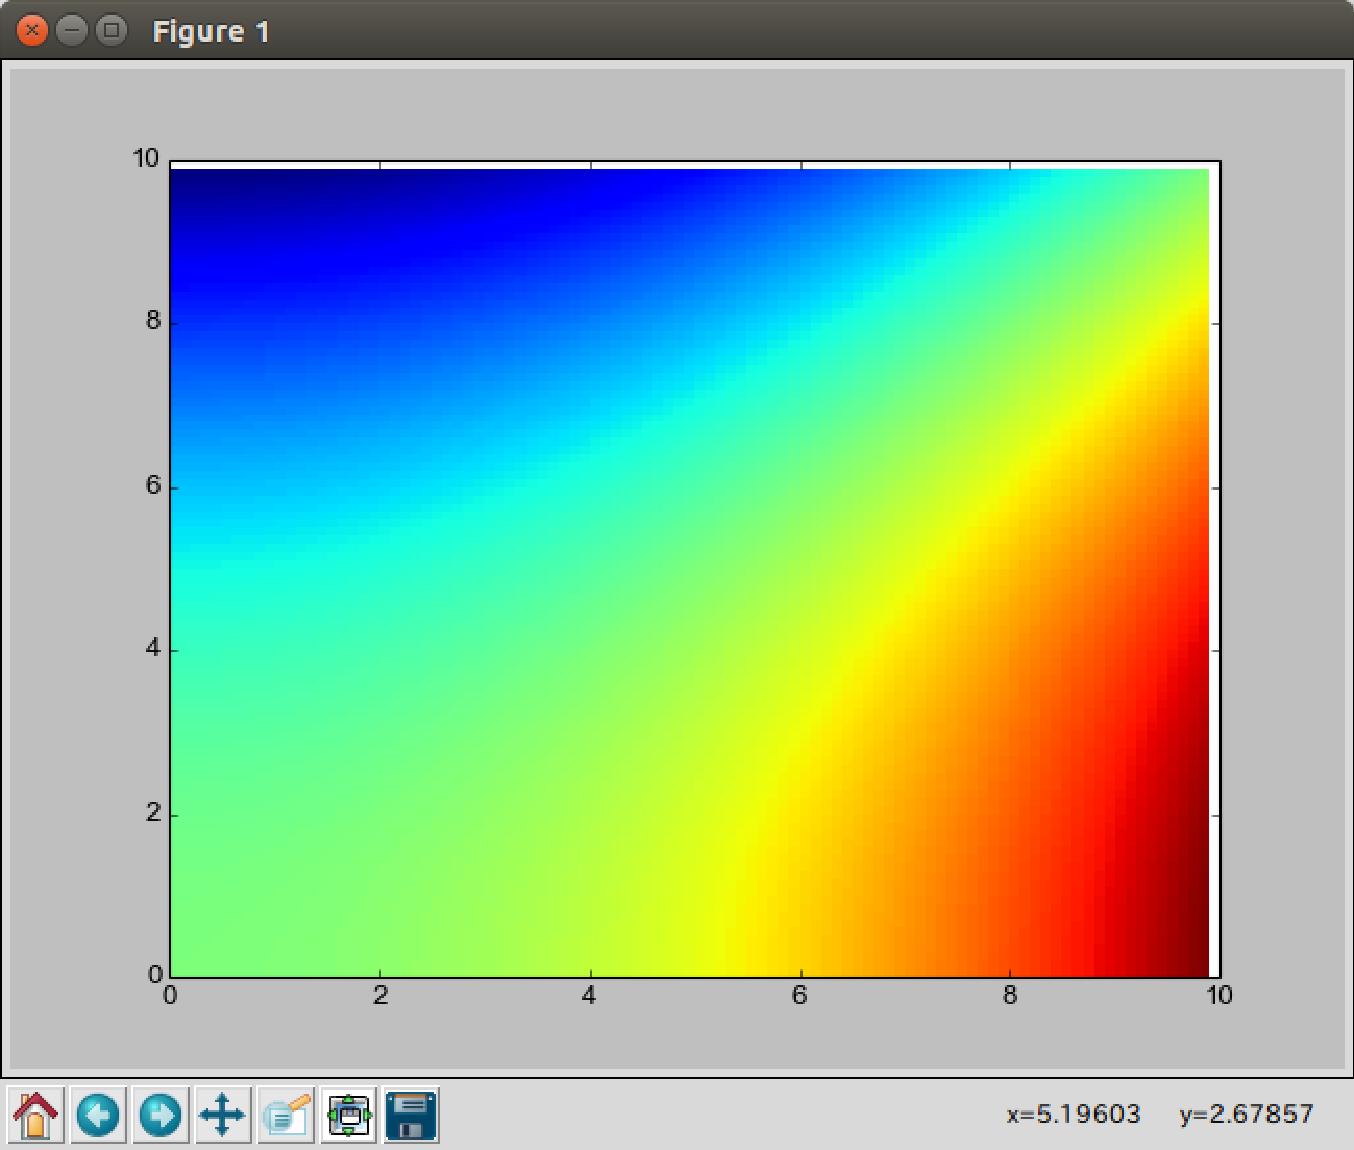
\includegraphics[width=0.5\textwidth]{out/pdf/img/pcolor.pdf}
\end{center}
\end{itemize}
\end{frame}




%%%%%%%%%%%%%%%%% %%%%%%%%%%%%%%%%% 
\begin{frame}[fragile]
\frametitle{もう少し柔軟なプロットの仕方}
\begin{itemize}
\item 複数のグラフを表示したい,3Dで表示したいという時には,
以下のスタイルで
\begin{lstlisting}
import matplotlib.pyplot as plt
fig = plt.figure() # windows全体
ax = fig.add_subplot(行数, 列数, 通し番号) # 一つのグラフ
ax.plot(...)
fig.show(...)
\end{lstlisting}

\item 例 (3x2のタイルで表示)
\begin{lstlisting}
import matplotlib.pyplot as plt
fig = plt.figure()
ax0 = fig.add_subplot(3,2,1) # @$\equiv$@ fig.add_subplot(321)
ax1 = fig.add_subplot(3,2,2) # @$\equiv$@ fig.add_subplot(322)
   ...
ax0.plot(...)
ax1.plot(...)
   ...
fig.show(...)
\end{lstlisting}
\end{itemize}
\end{frame}

%%%%%%%%%%%%%%%%% %%%%%%%%%%%%%%%%% 
\begin{frame}[fragile]
\frametitle{2変数関数($z = f(x, y)$)をプロットする.\aka{ただし3Dで}}

\begin{itemize}
\item 基本: {\tt plot}にかわる「それ用の」関数を使う
  \begin{itemize}
  \item \ao{\tt plot\_surface}
  \item \ao{\tt plot\_wireframe}
  \item etc.
  \end{itemize}

\item ただし,二つほどまじないが必要
\begin{lstlisting}
import matplotlib.pyplot as plt
import numpy as np
@\ao{\tt import mpl\_toolkits.mplot3d.axes3d}@
fig = plt.figure()
ax = fig.add_subplot(1,1,1, @\ao{\tt projection='3d'}@)
X = np.arange(0, 10, 0.1)
Y = np.arange(0, 10, 0.1)
X,Y = np.meshgrid(X, Y)
Z = X ** 2 - Y ** 2
ax.plot_surface(X, Y, Z)
plt.show()
\end{lstlisting}

\item \url{http://matplotlib.org/1.3.1/gallery.html#mplot3d}
参照

\end{itemize}
\end{frame}


%%%%%%%%%%%%%%%%% %%%%%%%%%%%%%%%%% 
\begin{frame}[fragile]
\frametitle{\aka{3D}でプロットの例}

\begin{itemize}
\item []
\begin{lstlisting}[basicstyle = \ttfamily\scriptsize]
import matplotlib.pyplot as plt
import numpy as np
import mpl_toolkits.mplot3d.axes3d
fig = plt.figure()
ax = fig.add_subplot(1,1,1, projection='3d')
X = np.arange(0, 10, 0.1)
Y = np.arange(0, 10, 0.1)
X,Y = np.meshgrid(X, Y)
Z = X ** 2 - Y ** 2
ax.plot_surface(X, Y, Z)
plt.show()
\end{lstlisting}

\item []
\begin{center}
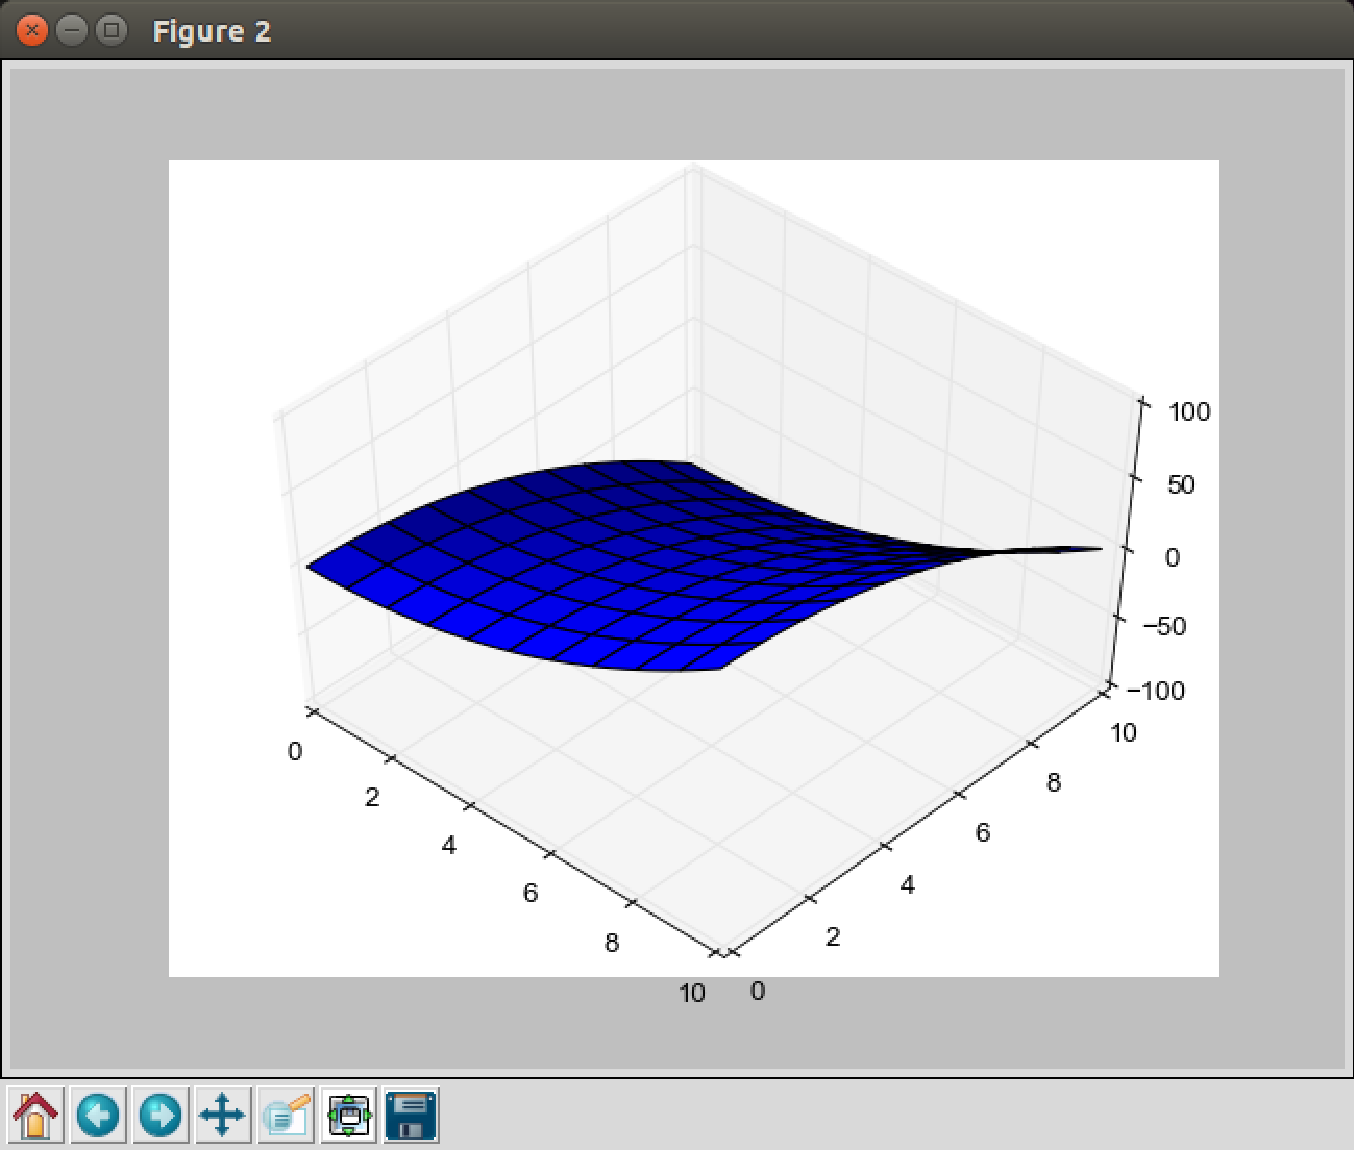
\includegraphics[width=0.5\textwidth]{out/pdf/img/plot_surface.pdf}
\end{center}
\end{itemize}
\end{frame}

%%%%%%%%%%%%%%%%% %%%%%%%%%%%%%%%%% 
\begin{frame}[fragile]
  \frametitle{Matplotlibでのアニメーション}
  \begin{itemize}
  \item 場が時間とともに発展するようなシミュレーションでは, 最終結果だけでなく, 途中も表示したい
  \item 最終結果がおかしい時,
    その原因を究明するためにも重要
  \item いくつか方法があるのだが,
    Jupyter環境のシステム上の問題で,
    動かないときが多い
  \end{itemize}
\end{frame}

%%%%%%%%%%%%%%%%% %%%%%%%%%%%%%%%%% 
\begin{frame}[fragile]
  \frametitle{例題}
  \begin{itemize}
  \item 問題:
  \[ y = \sin k x \quad (0 \leq x \leq 2\pi) \]
  のグラフを, $k = 1, 2, 3, \cdots 5$
  まで変えながら表示する
\item 復習: 固定した$k$ ($= 3$)
  について表示するだけでよいのなら以下
\begin{lstlisting}
import matplotlib.pyplot as plt
import numpy as np

x = np.linspace(0.0, 2.0 * np.pi, 100)
plt.plot(x, np.sin(3 * x))
plt.show()    
\end{lstlisting}

\begin{center}
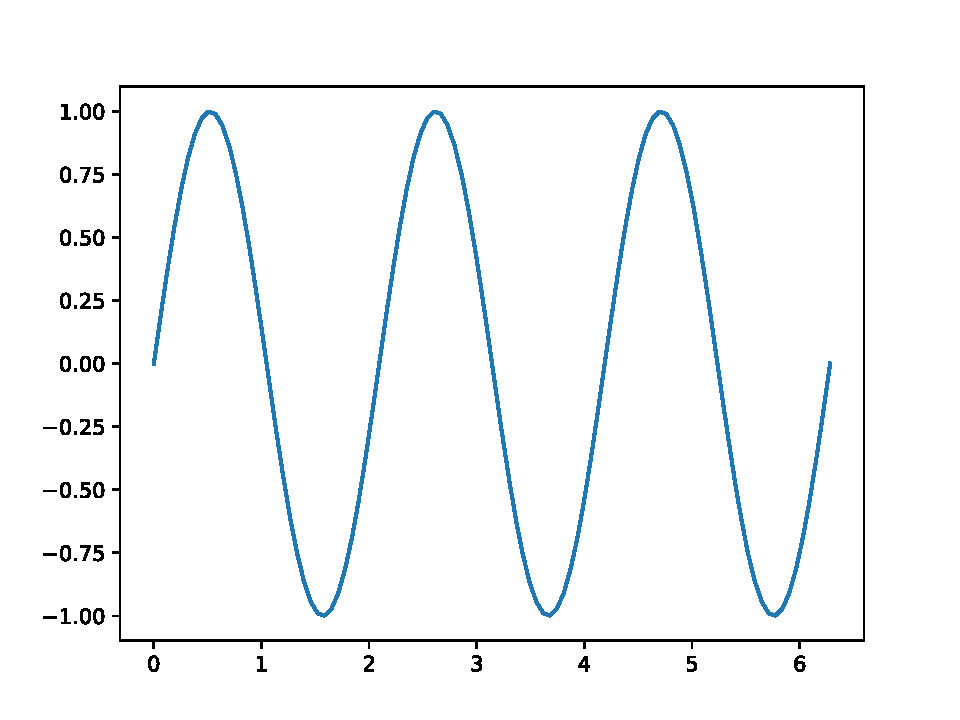
\includegraphics[width=0.5\textwidth]{out/pdf/svg/sinkx.pdf}  
\end{center}
  \end{itemize}
\end{frame}

%%%%%%%%%%%%%%%%% %%%%%%%%%%%%%%%%% 
\begin{frame}[fragile]
  \frametitle{一見それらしいけど不正解な例}
  \begin{itemize}
  \item []
\begin{lstlisting}
import matplotlib.pyplot as plt
import numpy as np

x = np.linspace(0.0, 2.0 * np.pi, 100)
for k in range(1, 6):
    plt.plot(x, np.sin(k * x))
plt.show()
\end{lstlisting}
\item おこること:
  5つのグラフが全部(重ねて)表示される

\begin{center}
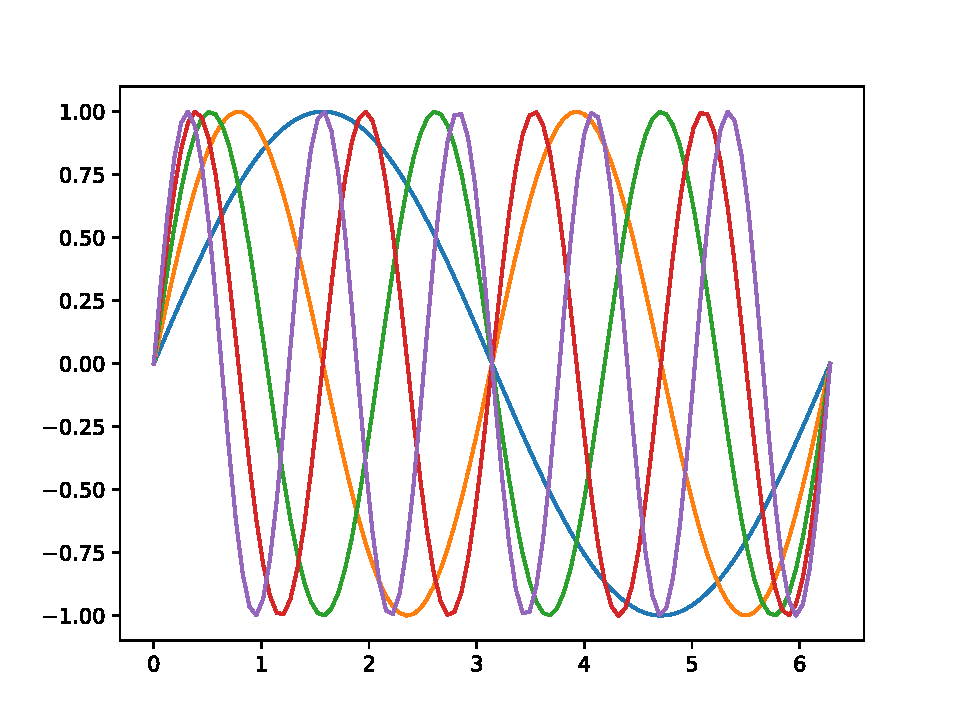
\includegraphics[width=0.5\textwidth]{out/pdf/svg/sinkx_all.pdf}  
\end{center}
  
\end{itemize}
\end{frame}


%%%%%%%%%%%%%%%%% %%%%%%%%%%%%%%%%% 
\begin{frame}[fragile]
  \frametitle{アニメーションの方法}
  \begin{itemize}
  \item 以下にアニメーションの方法を3つ述べるが,
    (田浦の調べた限り), Jupyter内でアニメーションができるのは,
    方法1だけ
  \item 他の方法はJupyter内では動かない
    \begin{itemize}
    \item (授業ではやっていない) pythonコマンドで実行すれば動く
    \end{itemize}
  \end{itemize}
\end{frame}

%%%%%%%%%%%%%%%%% %%%%%%%%%%%%%%%%% 
\begin{frame}[fragile]
  \frametitle{方法1}
  \begin{itemize}
  \item {\tt plt.plot(\ldots)}した結果は,
    「曲線」(のリスト)
  \item それらをリストに全て溜め($\ast$),
    {\tt animation.ArtistsAnimation}
    という関数に渡すと, それらを順にアニメーションしてくれる
  \item {\tt \%matplotlib notebook}というおまじないが必要
  \end{itemize}
\begin{center}
\begin{lstlisting}
@\ao{\tt \%matplotlib notebook}@
import matplotlib.pyplot as plt
import matplotlib.animation as animation
import numpy as np

x = np.linspace(0.0, 2.0 * np.pi, 100)
plots = []
for k in range(1, 6):
    @\ao{\tt plots.append}@(plt.plot(x, np.sin(k * x)))
@\ao{\tt a = animation.ArtistAnimation(plt.gcf(), plots, repeat=0)}@
plt.show()
\end{lstlisting}
\end{center}
\end{frame}

%%%%%%%%%%%%%%%%% %%%%%%%%%%%%%%%%% 
\begin{frame}[fragile]
  \frametitle{注意}
  \begin{itemize}
  \item 表示したい絵の数を無闇に大きくできない
  \item 例えば1万ステップのシミュレーションで全ステップの絵を表示するのは無謀
  \item リストの長さが適度になるように間引きする必要がある.
    例えば以下は表示する絵を{\tt max\_frames}個以下に押さえる方法
\begin{lstlisting}
n_steps = 123456
max_frames = 50
interval = math.ceil(n_steps / max_frames)
plots = []
for t in range(n_steps):
    if t % interval == 0:
        plots.append(...)
\end{lstlisting}
\item また, この方法の欠点: 計算が全て完了してから結果が初めて表示される
\item 計算しながら表示するには方法2, 3が必要だが, 残念ながらJupyter
  では動かない
\end{itemize}
\end{frame}

%%%%%%%%%%%%%%%%% %%%%%%%%%%%%%%%%% 
\begin{frame}[fragile]
  \frametitle{(参考) 方法2}
  \begin{itemize}
  \item 最初に一度{\tt plt.plot(\ldots)}
    して結果(曲線)を変数に入れる(\ao{$\ast$})
  \item その曲線のデータを{\tt set\_data}で変更(\ao{$\dagger$})
  \item 必要に応じて{\tt pause}で変更間隔を調整(\ao{$\dagger\dagger$})
  \item (田浦の知る限り) Jupyter内では動かない
    (pythonのコマンドラインでなら動く. 詳細不明)
  \end{itemize}
\begin{center}
\begin{lstlisting}
x = np.linspace(0.0, 2.0 * np.pi, 100)
for k in range(1, 6):
    if k == 1:
        @\ao{\tt [ line ] =}@ plt.plot(x, np.sin(k * x)) # (@\ao{$\ast$}@)
    else:
        @\ao{\tt line.set\_data}@(x, np.sin(k * x)) # (@\ao{$\dagger$}@)
    @\ao{\tt plt.pause}(0.1)@ # (@\ao{$\dagger\dagger$}@)
\end{lstlisting}
\end{center}

\begin{itemize}
\item 注: {\tt plt.plot(\ldots)}は, 描かれた曲線のリスト
  (普通は1要素)を返す; 実は一度に複数の曲線を描ける
\end{itemize}
\end{frame}

%%%%%%%%%%%%%%%%% %%%%%%%%%%%%%%%%% 
\begin{frame}[fragile]
  \frametitle{(参考) 方法3}
  \begin{itemize}
  \item (Jupyterでは動かない上, 難しいのであまり気にしないで)
  \item 方法2に似た方法. 但し以下のように「関数」にして,
    書き直したいものを{\tt yield}する($\ast$)
\begin{lstlisting}
def generate_plots():
    x = np.linspace(0.0, 2.0 * np.pi, 100)
    for k in range(1, 6):
        if k == 1:
            [line] = plt.plot(x, np.sin(k * x))
        else:
            line.set_data(x, np.sin(k * x))
        yield [line] # @($\ast$)@
\end{lstlisting}
\item その上で,
\begin{lstlisting}
@\ao{\tt animate\_iterator}@(@\ao{\tt generate\_plots()}@, interval=100)    
\end{lstlisting}
\item ただし{\tt animate\_iterator}は次ページ
\end{itemize}
\end{frame}

%%%%%%%%%%%%%%%%% %%%%%%%%%%%%%%%%% 
\begin{frame}[fragile]
  \frametitle{animate\_iterator}
  \begin{itemize}
  \item 以下はコピペでよい (説明は難しいので省略)
\begin{lstlisting}
import matplotlib.pyplot as plt
import matplotlib.animation as animation

def animate_iterator(iterator, **kwargs):
    def fun(*args):
        try:
            return next(iterator)
        except StopIteration:
            return []
    ani = animation.FuncAnimation(plt.gcf(), fun,
                                  **kwargs)
    plt.show()
\end{lstlisting}
  \end{itemize}
\end{frame}

%%%%%%%%%%%%%%%%% %%%%%%%%%%%%%%%%% 
\begin{frame}[fragile]
  \frametitle{2次元 (pcolor)の場合}
  \begin{itemize}
  \item 復習: アニメーションなしで静止画($z = y - \sin 3x$)を書くだけの例
    
\begin{lstlisting}
%matplotlib notebook
import matplotlib.pyplot as plt
import numpy as np
x = np.linspace(0.0, 1.0, 100)
y = np.linspace(0.0, 1.0, 100)
x,y = np.meshgrid(x, y)
plt.pcolor(x, y, np.sin(y - np.sin(3 * x)))
plt.show()      
\end{lstlisting}

\begin{center}
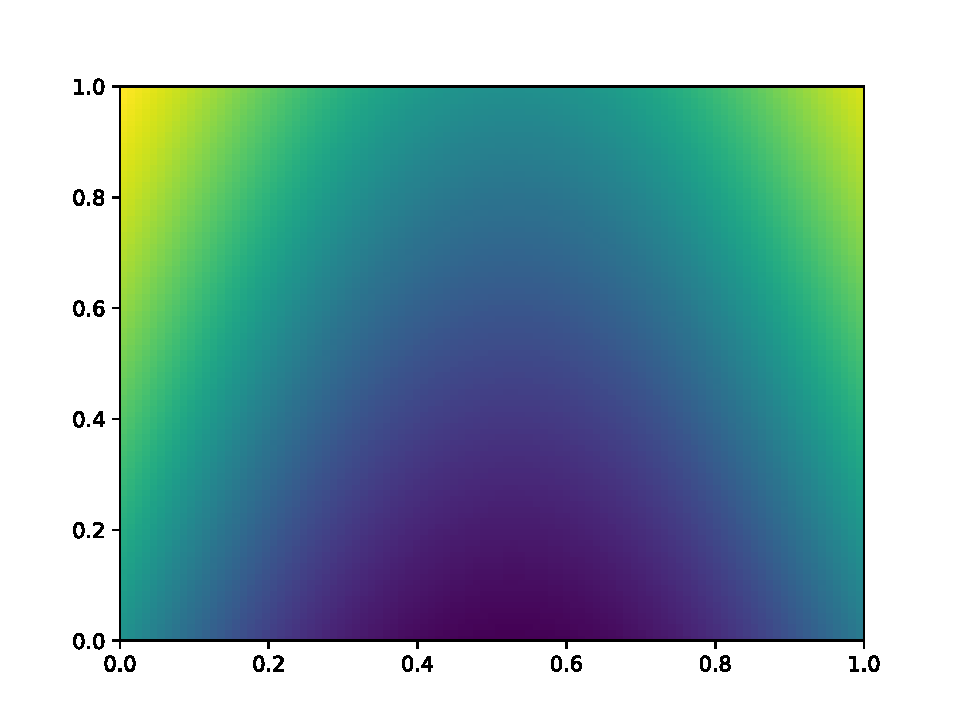
\includegraphics[width=0.4\textwidth]{out/pdf/svg/z_sinkx.pdf}
\end{center}

  \end{itemize}
\end{frame}

%%%%%%%%%%%%%%%%% %%%%%%%%%%%%%%%%% 
\begin{frame}[fragile]
  \frametitle{2次元 (pcolor) 方法1}
  \begin{itemize}
  \item 1次元と考え方は同じ({\tt pcolor}の結果をリストにためて,
    {\tt animation.ArtistAnimation}を呼び出す)
\begin{center}
\begin{lstlisting}
%matplotlib notebook
import matplotlib.pyplot as plt
import matplotlib.animation as animation
import numpy as np
x = np.linspace(0.0, 1.0, 100)
y = np.linspace(0.0, 1.0, 100)
x,y = np.meshgrid(x, y)
pcolors = []
for k in range(1, 20):
    pcolors.append(@\ao{\tt [ plt.pcolor(x,y,y-np.sin(k*x)) ]}@)
a = animation.ArtistAnimation(plt.gcf(), pcolors,
                              repeat=0)
plt.show()
\end{lstlisting}
\end{center}
\item {\tt plt.plot}の結果はリストだったが,
  (ややこしいことに){\tt plt.pcolor}の結果はリストではないので,
  自分で1要素のリストにする($\ast$)
\end{itemize}
\end{frame}

%%%%%%%%%%%%%%%%% %%%%%%%%%%%%%%%%% 
\begin{frame}[fragile]
  \frametitle{(参考) 2次元 (pcolor) 方法2}
  \begin{itemize}
  \item 注: Jupyterでは動かない
  \item 1次元({\tt plot})では{\tt set\_data}を呼んだが,
    2次元({\tt pcolor})では{\tt set\_array}を呼ぶ
  \item ややこしいことに, $z$座標のデータを1ずつ削り,
    かつ1次元配列に直して渡さないといけない(理由不明)
\begin{lstlisting}
import matplotlib.pyplot as plt
import numpy as np
x = np.linspace(0.0, 1.0, 100)
y = np.linspace(0.0, 1.0, 100)
x,y = np.meshgrid(x, y)
for k in range(1, 20):
    if k == 1:
        f = plt.pcolor(x, y, y - np.sin(k * x))
    else:
        f.@\ao{\tt set\_array(shrink1(y - np.sin(k * x)))}@
    plt.pause(0.1)
\end{lstlisting}
\item {\tt shrink1}は次ページ
  \end{itemize}
\end{frame}

%%%%%%%%%%%%%%%%% %%%%%%%%%%%%%%%%% 
\begin{frame}[fragile]
  \frametitle{shrink1}
  \begin{itemize}
  \item []
\begin{lstlisting}
def shrink1(z):
    m,n = z.shape
    return z[:m-1,:n-1].flatten()
\end{lstlisting}
\end{itemize}
\end{frame}

%%%%%%%%%%%%%%%%% %%%%%%%%%%%%%%%%% 
\begin{frame}[fragile]
  \frametitle{(参考) 2次元 (pcolor) 方法3}
  \begin{itemize}
  \item (Jupyterでは動かない上, 難しいのであまり気にしないで)
\begin{lstlisting}
def generate_pcolors():
    x = np.linspace(0.0, 1.0, 100)
    y = np.linspace(0.0, 1.0, 100)
    x,y = np.meshgrid(x, y)
    for k in range(1, 20):
        if k == 1:
            f = plt.pcolor(x, y, y - np.sin(k * x))
        else:
            f.set_array(shrink1(y - np.sin(k * x)))
        @\ao{\tt yield}@ [ f ]
\end{lstlisting}
\item その上で,
\begin{lstlisting}
animate_iterator(generate_pcolors(), interval=100)    
\end{lstlisting}
\item {\tt animate\_iterator}は1次元の場合と同じ
\end{itemize}
\end{frame}

\end{document}

